% Chapter 2

\chapter{Asymmetrische Verschlüsselung} % Chapter title

%\label{ch:examples} % For referencing the chapter elsewhere, use \autoref{ch:examples} 

Ein großes Problem der Kryptografie ist der Schlüsselaustausch, hierfür bietet die Asymmetrische Verschlüsselung eine Lösung.

%----------------------------------------------------------------------------------------

\section{Public Key}
Als Public Key wird der Teil des Schlüssel bezeichnet, der vom potentiellen Empfänger einer Nachricht frei zugänglich für jeden veröffentlich wird.
Dieser Teil des Schlüssels wird vom Absender der Nachricht benötigt, denn mit diesem Schlüssel wird die Nachricht vor dem versenden Verschlüsselt.
Nach diesem verschlüsselungsverfahren kann die Nachricht nur noch vom Empfänger mit dem Prvate Key gelesen (entschlüsselt) werden, nicht einmal der Empfänger kann jetzt noch auf die  Daten zugreifen.


%----------------------------------------------------------------------------------------

\section{Private Key}
Als Private Key wird der Teil des Schlüssels bezeichnet der nur dem Empfänger der Nachricht zur Verfügung steht und unter Verschluss gehalten wird.
Dieser Schlüssel dient dazu eingehende Nachrichten, die mit dem korrespondierenden Public Key verschlüsselt wurden wieder zu entschlüsseln.
Dies ist nur mit diesem Schlüssel möglich.

%------------------------------------------------

\section{Vor und Nachteile}
Bei der asymmetrischen Verschlüsselung ergeben die folgenden Vorteile gegenüber einer symmetrischen Verschlüsselung:
\begin{itemize}
    \item \textbf{Eliminierung des Schlüsselaustauschproblems} \\ Bei der symmetrischen Verschlüsselung gibt es keinen sicheren Kanal zur Schlüsselübergabe, bei der asymmetrischen Verschlüsselung benötigt die Schlüsselübergabe keinen Sicheren Übertragungskanal.\citep{paar:2016}
    \item \textbf{Die Anzahl der benötigten Schlüssel ist geringer} \\ Bei einer symmetrischen Verschlüsselung bräuchte jeder Benutzer von jedem Benutzer einen eigenen Schlüssel,
    \\bem asymmetrischen Verfahren reduziert sich die Schlüsselmenge auf je jeweilige Anzahl an Benutzern.\citep{paar:2016}
    \item \textbf{Authentizität} \\ Asymmetrische Verschlüsselung bietet zudem gegenüber der symmetrischen auch den Vorteil der Authentizität.
\end{itemize}
Nachteile die sich durch die asymmetrische Verschlüsselung ergeben:

\begin{itemize}
    \item \textbf{Ein erhöhter Rechenaufwand} \\ im vergleich zur symmetrischen Kryptografie.
\end{itemize}
%-------------------------------------------------

\section{Ablauf eine Asymmetrischen Verschlüsselung}
\begin{enumerate}
    \item Erstellen eines Schlüsselpaares bestehend aus Public und Private Key
    \item Veröffentlichen des Public Keys
    \item Der Absender lädt sich den Public Key vom Empfänger
    \item Der Absender verschlüsselt die zu übertragenden Daten mit dem Public Key des Empfängers
    \item Der Empfänger ist nun in der lage mithilfe seines passenden Private Keys die empfangene Nachricht zu entschlüsseln.
\end{enumerate}

\begin{figure}[ht]
	\centering
  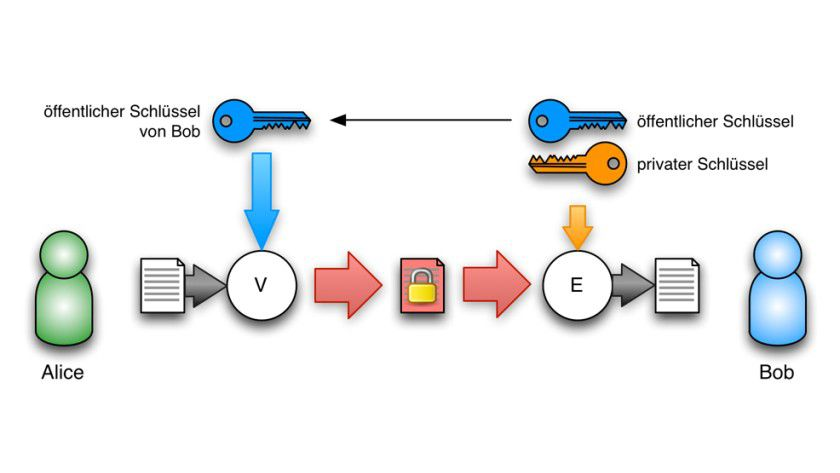
\includegraphics[width=12cm]{gfx/asymmetrisch.jpg}
	\caption{(V) Verschlüsseln\\(E) Entschlüsseln}
\end{figure}
\newpage
%--------------------------------------------------

\section{Implementierungen von asymmetrischer Verschlüsselung}

\begin{itemize}
    \item \textbf{S/MIME}\\steht für Secure Multipurpose Internet Mail Extension und ist ein Protokoll zum Verschlüsseln und Signieren von E-Mails.\citep{ERTEL:2020}
    \item \textbf{SSH}\\Secure Shell (SSH) ist eine Software um Rechner remote zu steuern und zu verwalten. Dabei wird die Verbindung durch den Einsatz von Public Key Verfahren verschlüsselt, ganz im gegensatz zu seinem Vorgänger Telnet dieser war unverschlüsselt.\citep{ERTEL:2020}
    \item \textbf{SSL}\\ Secure Socket Layer (SSL) ist ein Protokoll um TCP Verbindungen zwischen zwei Sockets zu verschlüsseln. 
    Dabei kommt eine Hybride Verschlüsselung zum Einsatz (mehr dazu später). SSL wurde später durch TLS (Transport Layer Security) abgelöst.\citep{ERTEL:2020}
    \item \textbf{VPN / IPsec}\\Virtual Private Networking und IP Security baut auf den Ideen und Grundlagen von SSL/TLS auf.
    Die Vorteile von IPsec beziehen sich auf die Verschlüsselung auf IP-Ebene (Layer 3) und nicht wie bei SSL/TSL auf Transport Ebene (Layer 4).
    Dadurch ist es IPsec möglich den kompletten Datenverkehr eines Netzwerks zu verschlüsseln. Ebenfalls müssen bestehende Anwendungen nicht verändert werden da IPsec unter der Transport Schicht (Layer 4) arbeitet.\citep{ERTEL:2020}
\end{itemize}